% Intended LaTeX compiler: pdflatex
\documentclass[dvipdfmx,10pt,presentation]{beamer}
\usepackage{amsmath, amssymb, bm}
\usepackage[utf8]{inputenc}
\usepackage{indentfirst}
\usepackage[normalem]{ulem}
\usepackage{longtable}
\usepackage{minted}
\usepackage{fancyvrb}
\usetheme{Berlin}
\usepackage[utf8]{inputenc}
\usepackage[T1]{fontenc}
\usepackage{graphicx}
\usepackage{grffile}
\usepackage{longtable}
\usepackage{wrapfig}
\usepackage{rotating}
\usepackage[normalem]{ulem}
\usepackage{amsmath}
\usepackage{textcomp}
\usepackage{amssymb}
\usepackage{capt-of}
\usepackage{hyperref}
\useoutertheme[subsection=false]{smoothbars}
\setbeamertemplate{footline}[page number]
\setbeamercolor{page number in head/foot}{fg=black}
\setbeamerfont{page number in head/foot}{size=\normalsize}
\usetheme{default}
\author{情報科学類3年 江畑 拓哉 (201611350)}
\date{}
\title{進捗報告}
\begin{document}

\maketitle
\begin{frame}{Outline}
\tableofcontents
\end{frame}

\section{要約}
\label{sec:orgbf22f9e}
\begin{frame}[allowframebreaks]{要約}
\begin{itemize}
\item Seq2Seq model について学習した。\\
\item 使用するライブラリを変更した。(それに伴い使用言語も変更)\\
\item 幾つかのモデルについて調べた。\\
\item 実験したいモデル\\
\item 今後の予定\\
\end{itemize}
\end{frame}

\section{Seq2Seq model について}
\label{sec:orgfa85d80}
\begin{frame}[allowframebreaks]{}
\begin{itemize}
\item 翻訳に多く使われている。\\
\item Q \& A 形式の一文が短い会話についても適用できる。\\
\item モデル図\\
\begin{center}
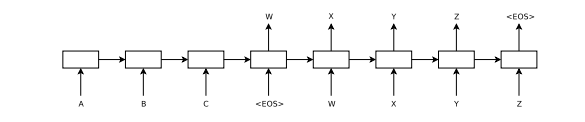
\includegraphics[width=.9\linewidth]{./seq2seq.png}
\end{center}
\item 参考文献\\
\href{https://web.stanford.edu/class/cs20si/2017/}{CS 20SI: Tensorflow for Deep Learning Research}\\
\href{https://www.researchgate.net/publication/323587007\_Deep\_Learning\_Based\_Chatbot\_Models}{Deep\_Learning\_Based\_Chatbot\_Models}\\
\end{itemize}
\end{frame}

\section{LSTM について}
\label{sec:org87191af}
\begin{frame}[allowframebreaks]{lstm}
\begin{itemize}
\item Long Short-Term Memory\\
\item 概図\\
\begin{center}
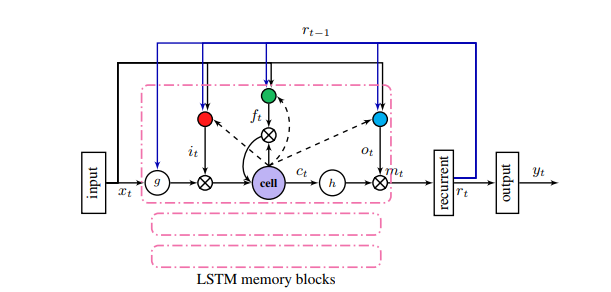
\includegraphics[width=.9\linewidth]{./lstm.png}
\end{center}
\end{itemize}
\end{frame}
\begin{frame}[allowframebreaks]{それぞれの要素に対する式}
\begin{align}
\bm{i}_t=\sigma(\bm{W}_{ix}\bm{x}_t + \bm{W}_{im}m_{t-1} + \bm{W}_{ic}\bm{c}_{t-1} + \bm{b}_i) \\ 
\bm{f}_t=\sigma(\bm{W}_{fx}\bm{x}_t + \bm{W}_{fm}m_{t-1} + \bm{W}_{fc}\bm{c}_{t-1} + \bm{b}_f) \\
\bm{c_t}=\bm{f}_t \odot \bm{c}_{t-1} + \bm{i}_t \odot g(\bm{W}_{cx}\bm{x}_t + \bm{W}_{cm}\bm{m}_{t-1} + \bm{b}_c) \\
\bm{o_t}=\sigma(\bm{W}_{ox}x_t + \bm{W}_{om}m_{t-1} + \bm{W}_{oc}\bm{c}_t + \bm{b}_o) \\
\bm{m}_t = \bm{o}_t \odot h(\bm{c}_t) \\
\bm{y}_t = \phi(\bm{W}_{ym}\bm{m}_t + \bm{b}_y)
\end{align}
\begin{align}
where\ &\bm{W}\ is\ weight \\
       &\bm{b}\ is\ bias \\
       &\odot\ is\ the\ element-wise\ product\ for\ vectors\\ 
       &\sigma\ is\ the sigmoid function \\
       &\phi \ is\ network\ output\ activation\ (e.g.\ softmax) \\
       &g,h \ is\ activation\ function\ (e.g. tanh)
\end{align}
なお、i は input 、f は forget 、o は output gate を表しており、 c は cell activation を示している。\\
※すべてのベクトルのサイズは等しい。\\
\begin{itemize}
\item 参考文献\\
\href{https://static.googleusercontent.com/media/research.google.com/ja//pubs/archive/43905.pdf}{Long Short-Term Memory Recurrent Neural Network Architectures for Large Scale Acoustic Modeling}\\
\end{itemize}
\end{frame}

\section{使用するライブラリを変更した}
\label{sec:org4370960}
\begin{frame}[fragile,allowframebreaks]{}
 \begin{itemize}
\item 以前は common lisp mgl を用いていたが、事情により撤回を余儀無くされた。\\
\begin{itemize}
\item 事情 Optimizer を絡ませずに lstm セルを回すことができない。\\
\end{itemize}
\begin{itemize}
\item 現在は TensorFlow を Hylang から利用している。\\
Python とTensorFlowの実行環境が入っていれば動く\\
(common lisp mgl の内部実装を熟読したが、頑張れば目的に対応する LSTM を実装できると思われる。\(\rightarrow\) それは卒研の目的とは外れてしまう。)\\
\item 現在ベースとなる Seq2Seq モデルそのものは完成(ほとんどドキュメントの翻訳に近い)しているが、実行にかなり時間がかかっており満足な結果を手に入れられていない。\\
リポジトリ \texttt{github.com/MokkeMeguru/hy-seq2seq-with-tensorflow}\\
\end{itemize}
\end{itemize}
\end{frame}


\section{新たに調べたモデル}
\label{sec:org3fb8263}
\begin{frame}[allowframebreaks]{}
\begin{itemize}
\item Doc2Vec\\
任意の長さの文章を分類するためのモデル。ある単語それぞれについてベクトル化を行い比較をする Word2Vec の文章版。類似の手法として Bag of Words という手法があるが、Doc2Vecは語順を考慮するという点や、単語の意味を表現するうことが出来るようになるらしいという点で有利。\\
文書ベクトルを並べた重み行列を用いて、入力となるある文章に対して最もふさわしい文書ベクトルを返す。\\
内部では PV-DM (文と文中の単語に固有のベクトルを与えて文に含まれる単語の予測を行う(語順を考慮している)) PV-DBOW (ランダムに抽出した文中の単語から、その文に含まれるだろう単語を予測する)が行われている。\\
既に文章からの感情分析において成果を出している。\\
\item Seq2Seq with Attention\\
Seq2Seq model を長文にも耐えられるように改良したもの。Decoder で最終的に取り出される hidden state を Encoder で毎回考慮させるようにしている。\\
\begin{center}
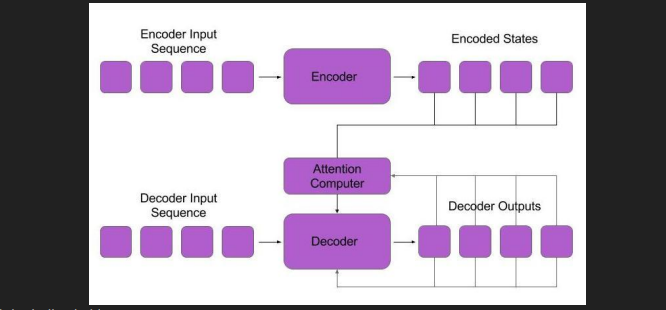
\includegraphics[width=.9\linewidth]{./attention.png}
\end{center}
\end{itemize}
\end{frame}
\begin{frame}[allowframebreaks]{}
\begin{itemize}
\item HRED\\
Seq2Seq model に文脈についての情報を与えるようにしたもの。長い会話を行えるようになる。\\
このため、RNNは Encoder Decoder に加え Context が必要になる。\\
\begin{center}
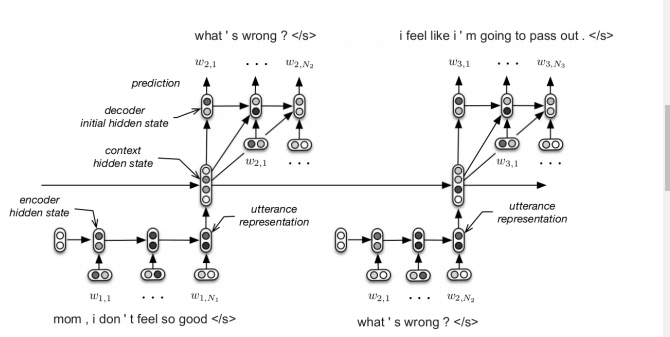
\includegraphics[width=.9\linewidth]{./hred.png}
\end{center}
\item 参考文献 \\
\href{https://cs.stanford.edu/\~quocle/paragraph\_vector.pdf}{Distributed Representations of Sentences and Documents}\\
\href{https://arxiv.org/pdf/1507.04808.pdf}{Building End-To-End Dialogue SystemsUsing Generative Hierarchical Neural Network Models}\\
\end{itemize}
\end{frame}
\section{実験したいモデル}
\label{sec:org7464197}
\begin{frame}[allowframebreaks]{}
\begin{itemize}
\item Doc2Vec でトピックごとの小さい問題に分割してそれぞれのトピックごとにSeq2Seq等を与えてみたい\\
=> 計算量が多く結果が満足に得られない/Doc2Vecで話者の気分を読み取ることができればそれに応じた返答が出来るのではないか?\\
\item Seq2Seq の部分を Seq2Seq with Attention や HRED に変えてみたい。\\
=> どの程度の差が生まれるのか比較を行いたい\\
\end{itemize}
\end{frame}
\section{今後の予定}
\label{sec:orgae67673}
\begin{frame}[allowframebreaks]{}
\begin{itemize}
\item TensorFlow に慣れる。\\
\item 実験を行い、結果データを得る。\\
\item 文体変換に関する論文を読む。(日本語の既存研究は見てきたが、あまりめぼしい物はなかった)  特徴として、すでに文章からの感情分析において成果を出している。\\
具体的には seq2seq を用いたものと GAN を用いたもの、Zero-Shot 変換を用いたものが論文としてあるので、この3つについて学習していきたい。\\
\item VHRED の論文を読む (HRED に確率成分を追加したものらしい)\\
\item 参考文献\\
\href{https://arxiv.org/pdf/1605.06069.pdf}{A Hierarchical Latent Variable Encoder-Decoder Model for Generating Dialogues}\\
\href{http://www.cs.tau.ac.il/\~joberant/teaching/advanced\_nlp\_spring\_2018/past\_projects/style\_transfer.pdf}{Deep Text Style Transfer}\\
\href{https://arxiv.org/pdf/1711.04731.pdf}{Zero-Shot Style Transfer in Text Using RecurrentNeural Networks}\\
\href{http://cl.naist.jp/\~yutaro-s/download/Shigeto\_NL222\_slides.pdf}{Ridge regression, hubness,and zero-shot learning}\\
\end{itemize}
\end{frame}
\end{document}
